\chapter{Related Work}
\label{chap:relWork}
\section*{Chapter Outline}
In this chapter we review prior studies related to the work carried out in this investigation, comparing the methods in which the work was conducted and the results found. We look at the state-of-the-art for a number of the domains and explain how we will use their findings in out investigations.


\section{Cortical Analysis}
% Discuss the work carried out by the Blue-Brain project in the extraction and analysis of the somatosensory cortex of a juvenile rat. Methodology they followed, information they amassed, topologies they discovered, and the various statistical information they collected.\\
% Short segment on the work related to LNP estimation, and how it differs to the estimation we need.
% \begin{itemize}
%     \item BBP, what they did, how they did it, and they data they supply.
%     \item Research into LNP estimation (STA STE etc)
% \end{itemize}

\begin{figure}
    \centering
    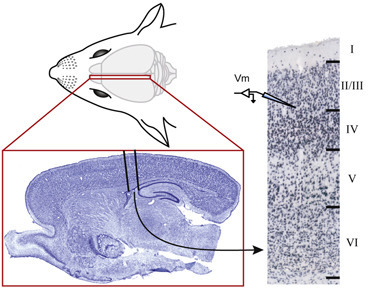
\includegraphics[width=0.65\textwidth]{03-Related_Work/ratbrain2.jpg}
    \caption{Segment of analysed brain \cite{reconSim}}
    \label{fig:ratbrain}
\end{figure}

\subsection{Source Data Extraction}
\label{chap:relwork:bbpData}
Previously mentioned was the work carried out by the Blue-Brain Project on the analysis of the somatosensory cortex of a juvenile rat, the result of which is used in this study as the source dataset for the simulated neurons \cite{reconSim}\cite{bbpTop}. This dataset comes from the reconstruction of a cortical column of the brain, where a small segment of about 0.3mm\textsuperscript{3} volume was extracted as shown in Figure \ref{fig:ratbrain}. This segment comprised of around 31,000 individual cells and about 36 million synaptic connections. The reconstruction comprised of two main parts: Reconstruction and classification of topologies; and reconstruction of the electrophysiology. For the reconstruction of topologies, 3-D reconstructions of neuronal morphologies were obtained from another study of $300\mu m$ thick brain slices \cite{markram1997physiology}. From these reconstructions, the morphologies were classified by whether they were excitatory or inhibitory, and further by the cortical layers into which they belonged. These were then correlated with the brain sample, and various methods were used to reconstruct the topologies found within the sample. As the samples consisted of brain samples, some of the topologies were truncated at the slice-edge. A number of "repair algorithms" were applied to reduce the negative effects of this truncation. These algorithms were based on first determining whether or not the topology truncation was indeed caused by the sample slice and not just the given shape of the topology. If the truncation was found to be caused by the sampling method, then a "regrowth" process was applied with a separate process depending on whether the regrowth was to a dendrite or an axon. The regrowth process takes into account the morphology of the cell, as well as the assumption of cell symmetry. While the process could not recover the exact morphology of the given sample, it was capable of recovering the cell to a "workable" state which fit the overall morphology, statistically speaking. Various corrections were also taken into account due to tissue shrinkage which may otherwise skew the reconstructed topologies.
\par
\begin{wrapfigure}{R}{0.45\textwidth}
    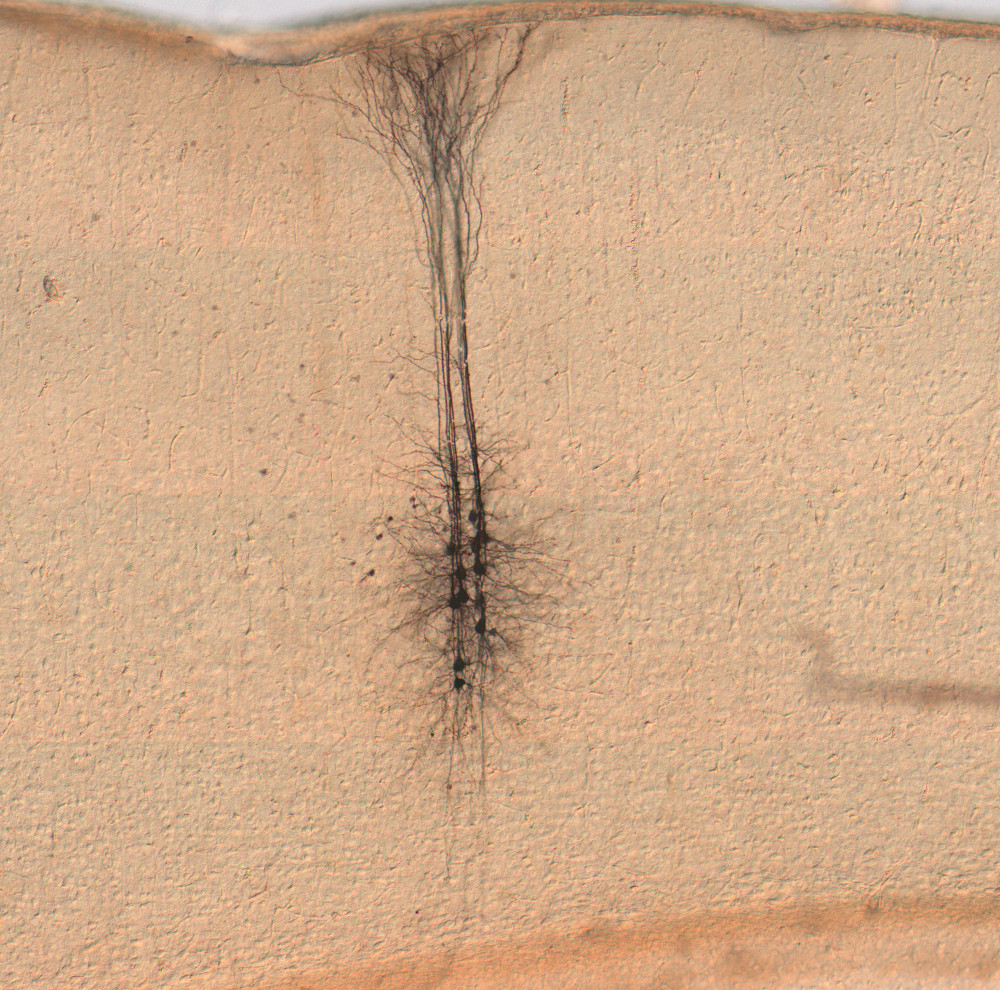
\includegraphics[width=0.45\textwidth]{03-Related_Work/l2brain.jpg}
    \caption{Sample of electrically-stimulated neurons \cite{nmcPortal}}
    \label{fig:leccyStimNeuron}
\end{wrapfigure}
To reconstruct the electrophysiology of the neurons in the brain sample, a number of in-vitro recordings were taken through the stimulus of a segment and expert-classifying the resultant waveform into one of 11 electrical types in table \ref{tab:e-type_table}. These stimulus protocols mostly dealt with the application of varying current and voltage levels over time and were all of a set of previously defined protocols: IDRest, APWaveform, and APThreshold \cite{wang2002anatomical}\cite{stimProtMark}). An image of a sample of electrically stimulated neurons is shown in Figure \ref{fig:leccyStimNeuron}.\\
Following the reconstruction of the neuron morphologies, electrophysiological properties, and overall network, analysis was done on the distribution of the various neuronal properties throughout the cortical segment. Of interest to us is the analysis of the pathways between any two neuron m-types. This was done by taking all pathways that exist between any 2 cell types (taking layer and m-type into account, disregarding e-type). For each pathway, the statistical values for parameters of the pathway anatomy, and for the path physiology were given. The parameters of the pathway anatomy largely deal with the connection in a physical sense, such as the mean/standard deviation (st.d.) of the number of synapses per connection, the mean/st.d. of the number of convergent/divergent neurons, as well as the connection probability. The parameters of the pathway physiology deal with the parameters of the pathway in a signal propagation sense, such as the mean/st.d. latency in the pathway. \\
\par
Following the reconstruction and analysis of the cortical column, the data was collected and published by the Blue Brain Project. A major contribution by the Blue Brain Project is the \emph{NMC Portal} \cite{nmcPortal}, an online portal which houses all data and publications undertaken in this research. The portal has a number of interactive "fact-sheets" which outline the analysed pathways between neurons, as well as renderings of the full reconstruction and videos of the network being simulated.\\
Through the portal it is also possible to obtain a copy of all experimental data. For each reconstructed cell (including layer, m-type, and e-type, along sub-variations) all data is supplied to replicate the neuronal simulation. This includes 3-D morphology descriptors, electrophysical mechanisms for the synapse types, as well as a list of all synapses (with parameters) available on the cell's dendrites. The cellular data files are discussed later for the simulation of the cells.\\
The portal also supplies the pathway information (physiology and anatomy) for each neuron-to-neuron pathway in JSON format. The JSON (Javascript Object Notation) format is a human-readable data format which represents a hierarchical set of key-value blocks. It can be used to specify a hierarchy of objects, each with a set of named parameters and associated values. In this format it is possible to quickly load the statistical data for analysis. A sample JSON data entry for pathway physiology can be found in \ref{ap:pathPhys}. This, again, is discussed in more detail later.

\subsection{Application of the LNP Model}
In Section \ref{chap:back:neurons} we discussed the Linear-Nonlinear-Poisson (LNP) cascade model of neuron characterisation. This model has been used experimentally in the analysis of the response of neurons in retinal ganglion cells \cite{lnpInBrain}. Here, the linear-nonlinear segments of the LNP model are joined in concept to be treated as a single block that takes an input stimulus and produces a response function which gives the output spike-rate. This response function is defined by
\begin{equation}
    \label{rsLnp}
    R(\vec{s}) = N(\vec{w} \cdot \vec{s})
\end{equation}
where $\vec{s}$ is the input stimulus, $\vec{w}$ is a vector of the same dimension of $\vec{s}$ representing the linear filter, and $N()$ is a function representing the non-linearity. The reason the linear-nonlinear segments are joined is that it becomes easier to predict $R(s)$ if this assumption is made, as this way the \emph{Spike-triggered average} (STA) metric can be used. The STA is defined as the average stimulus that leads to an output spike, and is calculated by taking a sum of the input stimulus values for each time-step that led to an output spike, divided by the total number of spikes, i.e.
\begin{equation}
    \label{staLnp}
    \vec{a} = \frac{ \sum_{t=1}^{T}\vec{s_{t}}f_{t}}{ \sum_{t=1}^{T}f_{t} }
\end{equation}
where $\vec{a}$ is the spike-triggered average, $\vec{s_{t}}$ is the input stimulus vector at time $t$, and $f_{t}$ is the output spike count at time-bin $t$. In this case, the STA is calculated over all time-steps from 0 to T, where T is the length of the recording period. It can be shown that $\vec{a} \propto \vec{w}$, and for the calculation of the nonlinearity function $N$ it is taken that $\vec{a} = \vec{w}$. A \emph{generator} signal is then defined as $\bar{g} \approx \vec{a} \cdot \vec{s_{t}}$, i.e. the "closeness" of the input stimulus to the precalculated STA. Following this, it was found that N could be calculated using the approximation
\begin{equation}
    \label{nonlinLnp}
    N(x) \approx \alpha C(\beta x + \gamma )
\end{equation}
where $\alpha$ is the maximum firing rate for the given neuron, $\beta$ is the sensitivity of the nonlinearity function to the generator function $\bar{g}$, and $\gamma$ is the "maintained drive to the cell", used to produce spikes in the absence of input stimulus. These parameters are selected to best fit the cell output based on least squared error. In testing, it was found that this method produced neuronal models with a root-mean square (RMS) difference of about 0.384 spikes per bin versus the observed actual output spike train. It was also noted that the RMS difference of averaging prior output results from the cell analysis was about 0.382 spikes per bin, indicating that the LNP-estimated model was nearly as accurate as the results from physically measuring the voltage at the cell.


\section{Neuronal-Link Parameters}
\label{chap:relWork:nrnLinkParams}
% TODO: Short section discussing the theoretical and experimental related work on analysing the mutual information of a neuronal link, and how its different to what we did.
% \begin{itemize}
%     \item Look at different papers describing the mutual information of a synaptic connection (i.e. the complex ones)
%     \item Mention the network tomography paper on delay estimation
%     \item Maybe find another bit of research on delay estimation with cross-correlation
% \end{itemize}
In Eq. \ref{eq:mutualInf} we stated the expression of the mutual information of a discrete memoryless system and stated that this was one of the models of expressing the metric, with other models fitting better to other types of systems. Prior work investigating the mutual information in a neural link has expressed the entropy of a source through the time-binning of the spike train, and defining the set of possible symbols as the possible neural response within the time period \cite{spikeTrainInfo}. For a window of length $T$ and a time-bin of length $\Delta\tau$, this leads to a symbol set of size $N = T/\Delta\tau$. Using the expression for entropy given in eq. \ref{eq:entropyDiscr}, the "naive" estimate of the neural entropy is given as
\begin{equation}
    \label{eq:naiveEntr}
    H(X)_{naive} = -\sum_{i=0}^{N}p(x_{i})\log_{2}(p(x_{i}))
\end{equation}
where X is the random variable, and $x_{i}$ is some symbol in the symbol set. The issue presented with this model is that a large data set is required to converge on a true entropy value. A possible workaround that was presented is to instead calculate a lower and upper bound on the entropy value which is robust regardless of dataset length. The lower bound presented is given by
\begin{equation}
    \label{eq:lowerEntr}
    H(X)_{lower} = -\sum_{N_{sp}}{P(N_{sp}) \times \log_{2}\left[P(N_{sp})\frac{2n_{c}(N_{sp})}{N_{obs}(N_{sp})[N_{obs}(N_{sp})-1]}\right]}
\end{equation}
where $N_{sp}$ is the "distribution of words with a fixed spike count", $n_{c}(N_{sp})$ is the "number of coincidences observed among the words with $N_{sp}$ spikes, $N_{obs}(N_{sp})$ is the "total number of occurrences of words with $N_{sp}$ spikes", and
$P(N_{sp})$ is the "fraction of words with $N_{sp}$ spikes". Similarly, an upper limit on the entropy was expressed as
\begin{equation}
    \label{eq:upperEntr}
    H(X) \leq \frac{1}{\Delta\tau}\left[H_{T+\delta\tau}(X) - H_{T}(X)( \right]
\end{equation}
for all T, where $H_{M}(X)$ is the entropy of X for some window length M. From this definition of entropy, it was found that the information rate (i.e. the mutual information) of the system increased with an increasing entropy, as expected.

%TODO:\textbf{Might add more here if there's enough time: delay estimation with cross correlation; and the fourier-transform tomography delay stuff}

\section{Classification of Neuronal Circuits}
% Discussion of Alaa's work (among others) on the classification of neurons in neuronal circuits. Also discuss topology discovery.
% \begin{itemize}
%     \item Alaa's work on cell classification
%     \item Alaa's work on topology discovery
%     \item Some more research here on other work in this area
% \end{itemize}



Prior work has investigated the classification of network parameters given simulated endpoint data \cite{ekkyProj}. A layer 5 cell was selected (layer 5, DBC m-type, cAC e-type), and 4 different combinations of 4 pre-synaptic cell m-types were selected: \{\{PC,PC,LBC,IPC\}, \{MC, SP, STPC, BP\}, \{PC, NBC, UTPC, UTPC\}, and \{PC, PC, STPC, IPC\}\}. The post-synaptic cell was then stimulated, and the soma-membrane voltage was measured for each of the pre-synaptic groups. The features used in this classification model were the frequency, delay, and number of spikes, along with the voltage-vs-time measurement of soma-membrane potential, and the average power spectral density. The overall accuracy of this classification model was about 83\%, with the model performing well for all pre-synaptic groups other than \{PC,PC,LBC,IPC\}.
\par
As well as cell-group classification, a topology-discovery classifier was also investigated. The intention of this classifier is to estimate the type of topology from which the measurements were taken, based on a small set of topology-type classes. In this case, the topology classes selected were {4-leaf star, 2-leaf star, and individual}. Here, "individual" means a single cell, while the star topologies are based on a network with a single central node, and a number of connected leaf nodes surrounding the centre (this is discussed in more detail later). The topologies investigated were relatively small and the classifier achieved accuracies as high as 99.37\% when classifying the 2-leaf and 4-leaf topologies through the use of decision trees. \\
While the research conducted focused mainly on a relatively small number of neurons, we expand on this by investigating similar types of classification with more complex sets of classes, such as with the full set of cell-possibilities.\\

%TODO:\textbf{Might add more here if there's enough time: theres been other research into cell-type classification that would fit well here.}

% As well as this, we hope to infer more link-level characteristics of the network rather than only
% classification of the circuit type, which could be done through the use of theory from network
% tomography.

% \par
% Network tomography deals with the inference of network characteristics such as link-by-link
% loss rates and delay distributions from a finite number of endpoint measurements [7]. It is
% achieved by treating the problem as a linear model, y = Aθ +  with known routing tables (A,
% a matrix) and measured endpoint data (y, a vector), solving for a vector of packet parameters
% (θ). The final term, , represents the noise term of the system (such as perturbations in the
% packet parameters). In many network systems, the size of the matrix tends to be quite large,
% and so solving for the packet parameters is non-trivial. As it is a linear problem, inversion
% is used which has well-documented solutions for possible approaches to solving the problem.
% In general this comes down to either solving for a linear combination of the parameters, or
% solving through the use of regularisation to bring identifiability. In this project we will apply
% the theory of network tomography to some common cortical circuit topologies in order to infer
% these link-level characteristics.

% \par 

% The circuit topologies that will be later investigated are based on the findings of [5] which
% investigated the structure of the networks found in the reconstructed juvenile rat somatosensory
% neocortex. Despite this reconstruction being comprised of roughly 31,000 cells, it was found that
% the average separation of any two cells was 2.5 synapses, indicating a small-work topology. This
% indicates a large degree of inter-layer connectivity, which is a point that will be investigated
% in our research during the construction of the various circuits. The article notes that the
% large-scale network properties analysed were likely the result of the constraints of the cortical
% reconstruction itself (such as the limitations of the cortical slices reducing the extent to which
% the axons were captured). This, however, should not be a major issue in our research as we will
% be dealing with circuits at a scale far below that of the full reconstruction and so the findings
% of the article dealing with smaller-scale network properties will be applicable.